\subsection{Validation of the methodology}

% \subsection{Testing is simulated scenario}\label{sec:synth}
In order to validate our algorithms we devised a simulated touching environment,
where we performed a number of tests on 9 everyday objects, like bowls, pots, spoons and mugs.
In order to have a ground truth for our tests we used complete point clouds and polygonal meshes of
such objects, those are visible in Figure~\ref{fig:meshes}.

\begin{figure}[htb]
    \centering
    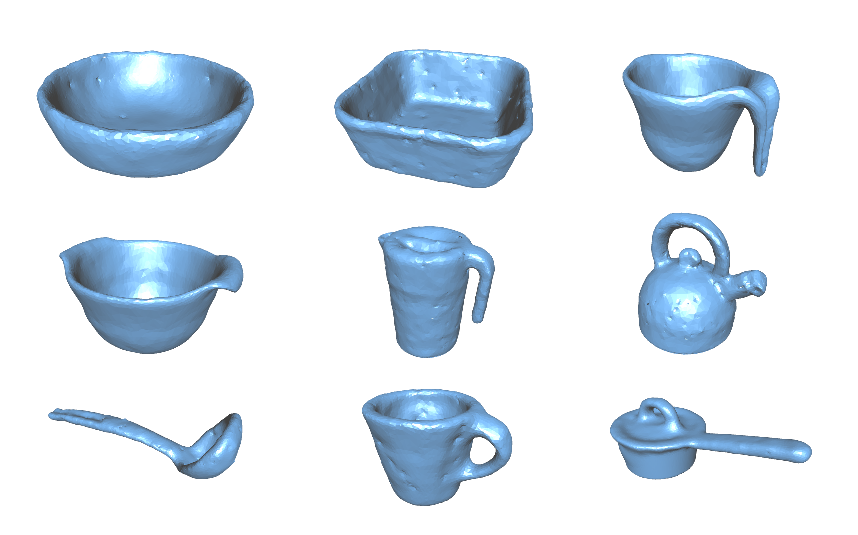
\includegraphics[width=0.95\columnwidth]{meshes.eps}
    \caption{Object meshes used as ground truth for our tests. From top to bottom and from left
    to right: bowlA, bowlB, containerA, containerB, jug, kettle, spoon, mug and pot.}
    \label{fig:meshes}
\end{figure}

These data represents full recontructed shapes and were obtained by means of a common
RGBD sensor and a turn table. The meshes created this way are used as ground thruth 
comparison for shapes reconstructed by our algorithm and at the same time,
are used to extract  partial view point clouds to set as initial training
data ($\mathcal{S}^0$), for our Gaussian Process regression, see Sec.~\ref{sec:gpis}.
It is worth nothing, that the meshes obtained this way are affected by sensor measurements noise 
and they don't perfectly represents the real object shapes. However this is no concern to us, because also the
training sets used in our validations are obtained from the same meshes, thus estimations and ground truth are
consistent with each other.

Each test we performed encloses a full object shape reconstruction and it's carried over
by iterating our \textsc{GPAtlasRRT} algorithm, Alg.~\ref{alg:strategy}~in~Sec.~\ref{sec:solution},
until the shape is predicted with desired variance $\mathbb{V}_{\max} = 0.1$.
% find a solution path that defines the best next tactile action to perform, until

The best next tactile action to perform at each iteration is simulated in our
environment by using  raycasting techniques towards the ground truth mesh.
Rays are uniquely defined by a chart center, as pivot point, and its normal, as direction.
Thus we can define  ray-mesh intersections as touches, i.e. points on surface, and no intersections
as points outside the surface. These new points are used to update the training set
and the GP model, from which a new \textsc{GPAtlasRRT} iteration can take place. 

In order to broaden our tests, we adopted three different tactile actions for each object, consequently forming 
three test groups, for a total of 27 full shape reconstructions. Each test group is described as follows:
\begin{asparadesc}
    \item[Random Touch], for the first test group we ignored the \textsc{GPAtlasRRT} solution path and 
        we just touched a random point on the GP manifold, with the raycasting technique described above.
        The random touching is repeated until the reconstructed shape is correctly predicted with
        desired variance of $0.1$.
        It is worth nothing that we expected these tests to take a fairly high amount of touches
        in order to recontruct the shape and they were performed as a comparison for our method.
        Test results are visible in Table~\ref{tab:test1}.
    \item[Single Poking], for the second test group we actually begin using the \textsc{GPAtlasRRT} solution by
        poking the last chart identified by the path. I.e. we used the raytracing technique applied to the last
        chart of the solution path, performing a touch were the algorithm tells us to go.
        Convergence criteria are the same as the previous test, thus we repeat tactile actions
        until the shape is fully reconstructed. Results in Table~\ref{tab:test2} shows a significant reduction
        in number of tactile actions required, in order to reach requested shape variance.
    \item[Sliding Touch],  for the  final test  category we  decided to  use the
    \textsc{GPAtlasRRT}  full solution  path. Starting  from the  root chart  we
    begin raytracing towards the ground truth mesh and from the touched point we
    reininterpolate a  path towards the next  chart. The new path  is raycasted
    again, while it is being traversed, yielding another point to generate a new interpolated path, and so
    on until we traverse all the charts in the path and we reach the tip of the atlas branch.
    With this technique we mimic a probe that is trying to slide across the surface,
    while trying to maintain contact with it. As the virtual probe slides we can discover
    a fairly significant amount of points on the surface and thus we can add more points to the trainging set
    with a single touch action. For this very reason we expected this test to be the most performing among the three,
    in terms of steps requirements, but also in terms quality of the reconstructed shape.
    Table~\ref{tab:test3} shows this test results, which met our expectations.
\end{asparadesc}
\begin{table}
    \centering
    \begin{tabularx}{0.95\columnwidth}{lccccccr}
        \toprule
        Object &&& & & Steps && RMSE \\
        \midrule
        bowlA &&& & &67 && 0.0025\\
        bowlB &&& & &38 && 0.0038\\
        containerA &&&&& 124 && 0.0033\\
        containerB &&&&& 68 && 0.0062\\
        jug &&&&& 106 && 0.0027\\
        kettle &&&&& 98 && 0.0031\\
        spoon &&&&& 35 && 0.0058\\
        mug &&&&& 238 && 0.0017\\
        pot &&&&& 33 && 0.0035\\
        \midrule
        \textbf{Mean} &&&&& $\sim$\textbf{90} && \textbf{0.0036}\\
        \bottomrule
    \end{tabularx}
    \caption{Random Touch test results. Steps column refers to the required number of
    tactile actions needed to reach the requested variance of $0.1$, while RMSE column shows
the Root Mean Squared Error calculated from the final predicted shape on the ground truth mesh.}
    \label{tab:test1}
\end{table}
\begin{table}
    \centering
    \begin{tabularx}{0.95\columnwidth}{lccccccr}
        \toprule
        Object &&& & & Steps && RMSE \\
        \midrule
        bowlA &&& & &27 && 0.0023\\
        bowlB &&& & &18 && 0.0036\\
        containerA &&&&& 20 && 0.0035\\
        containerB &&&&& 19 && 0.0043\\
        jug &&&&& 20 && 0.003\\
        kettle &&&&& 17 && 0.0032\\
        spoon &&&&& 10 && 0.0055\\
        mug &&&&& 28 && 0.0020\\
        pot &&&&& 12 && 0.0032\\
        \midrule
        \textbf{Mean} &&&&& $\sim$\textbf{19} && \textbf{0.0034}\\
        \bottomrule
    \end{tabularx}
    \caption{Single Poking test results. Again, steps column refers to the required
    number of tactile actions needed and RMSE column is the Root Mean Squared Error between
    the predicted shape and the actual ground truth mesh.}
    \label{tab:test2}
\end{table}
\begin{table}
    \centering
    \begin{tabularx}{0.95\columnwidth}{lccccccr}
        \toprule
        Object & & &&& Steps && RMSE \\
        \midrule
        bowlA &&& & &8 && 0.0015\\
        bowlB & &&& &5 && 0.0028\\
        containerA &&&&& 11 && 0.0028\\
        containerB &&&&& 8 && 0.0026\\
        jug &&&&& 9 && 0.0025\\
        kettle &&&&& 9 && 0.0029\\
        spoon &&&&& 8 && 0.0031\\
        mug &&&&& 12 && 0.0018\\
        pot &&&&& 6 && 0.0028\\
        \midrule
        \textbf{Mean} &&&&& $\sim$\textbf{8} && \textbf{0.0025}\\
        \bottomrule
    \end{tabularx}
    \caption{Sliding Touch test results. Steps column indicates the amount of tactile action required, RMSE
    column is the Root Mean Square Error between reconstructed shape and ground truth mesh. This method clearly
outperforms the others, in terms of efficiency and quality of the shape produced.}
    \label{tab:test3}
\end{table}

The three set of experiments clearly shows the superiority of our method in terms of number of required steps
and in terms of quality of produced mesh. As a final benchmarking, Table~\ref{tab:comp} summarizes the comparison
between the test methods and Fig.~\ref{fig:shapecomp} shows some  of the \textsc{GPAtlasRRT} Sliding Touch reconstructed shapes with
the ground truth meshes next to them.
\begin{table}
    \centering
    \begin{tabularx}{0.95\columnwidth}{lccccr}
        \toprule
        Tests  &&& Mean Steps && Mean RMSE \\
        \midrule
        Random Touch & & &90 && 0.0036\\
        Single Poking && &19 && 0.0034\\
        \textbf{Sliding Touch} &&& \textbf{8} && \textbf{0.0025}\\
        \bottomrule
    \end{tabularx}
    \caption{Comparison between test results. GPAtlasRRT with Sliding Touch outperforms other methods in terms
    of efficiency and precision.}
    \label{tab:comp}
\end{table}
\begin{figure}[htb]
    \centering
    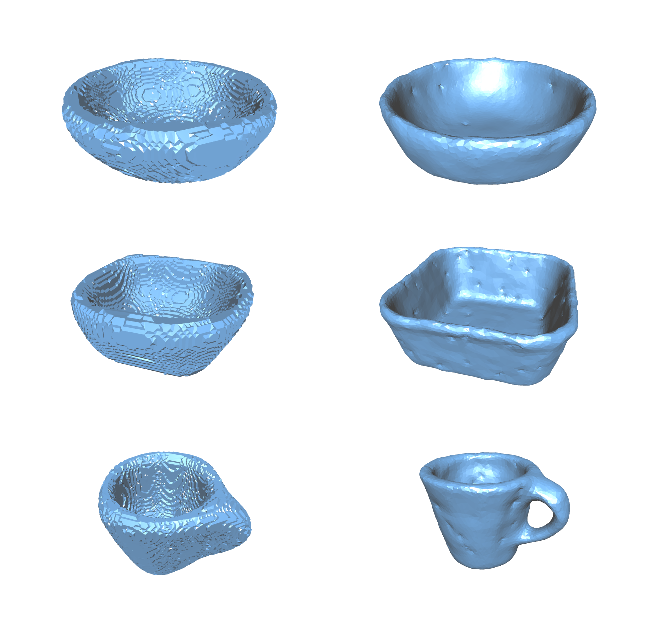
\includegraphics[width=0.95\columnwidth]{comparison.eps}
    \caption{Comparison of a few reconstructed shapes with the ground truth meshes. Left column are obtained with our GPAtlasRRT with Sliding Touch, while right column are the corresponding ground truth meshes.}
    \label{fig:shapecomp}
\end{figure}

Additionaly, while we performed our validation, we also recorded some videos of shape reconstructions, visible online at \texttt{https://goo.gl/4GKYTp}.
\subsection{Testing on a real scenario}
\label{sec:real}

%As stated in Secs.~\ref{sec:equipment}~and~\ref{sec:limitations}, a partial point cloud
%of a segmented object is required in order to get observation points for the initial
%surface estimation and speed up the shape modeling.
%\citet[Sec.~III.A]{Hudson2012Endtoend}  provides  good   candidate algorithms  for  object
%segmentation  that are  well oriented  to  object grasp,  manipulation, and  for
%our  purposes, exploration.  In fact,  the  combination of  their ``Table  Plane
%Estimation''  with their  ``Volume-Based  Segmentation''  yields the  ubiquituos
%tabletop object segmentation \citep{TabletopObjectDetector}. However, to improve
%the  rechability  of the  exploration,  we  prefer to  hold  the  object in  one
%hand-arm system and explore with the other, as described in Sec.~\ref{sec:scope}.
%\todo[]{Descrition in section 3 is missing. Also should point to the subsection, not the section.}
%Thus,  our selected  approach  for  object segmentation  is  simpler than  those
%approaches.  The  difficulties are  in  measuring  the  configuration of  a  soft
%and  adaptable  hand, like the Pisa/IIT SoftHand,
%\todo[]{I think we should cite some softhand paper here.}
%that  keeps  the  object  in  position  to  filter  out
%the  points  belonging  to  the  hand-arm system.  For  this  purpose,  one  can
%rely in  body-type measurements  instead of  traditional encoders,  as described
%in~\citet{Santaera2015Lowcost}.

We assume that the robot holds the object in its left hand. This allows the robot to move the object in a position where a snapshot of the object can be taken from the RGB-D camera disposed on its chest. \todo[]{we should put here a picture of Vito observing the object and what it is visible in simulation}
The acquired point cloud is an incomplete, noisy observation of the object, but it also likely contains other elements like, for example, the robot's hand-arm system as well as part of the background. 

Our propose solution to isolate the object's point cloud is to firstly utilise the robot's proprioception to remove the parts of the point cloud that most likely belong to the robot's body. However, measuring  the  configuration of  a  soft and  adaptable hand, like the Pisa/IIT SoftHand, is a challenging problem. For this purpose, we rely on a similar solution proposed by~\citet{Santaera2015Lowcost}; a sensorised glove which allows us to estimate the kinematic configuration of the soft hand at any time.

Once the hand-arm  system pose is measured, then
some   passthrough filters with slightly  scaled bounding boxes of  the robot
geometry  are used  to obtain  a  point cloud  of  the object  isolated from  the
robot. The scaling factor $\kappa$ is used to account for any incertainties that might
be present in the robot state or in the point cloud measurements. 
By slightly enlarging the robot bounding boxes we make sure that the object is correctly
separated from it, at the cost of losing some object points on the hand-object edge.

A further box filter is then applied to isolate the object from the rest of the scene,
thus obtaining a segmented object point cloud. 
Finally the obtained point cloud is further resampled to reduce the overall point
density, mantaining the object geometrical properties, while at the same time
improving Gaussian Process computation speed. 
\todo[]{Perhaps voxel grid description can be omitted}

This last downsampling step is performed with a Voxel Grid Filter, which, after
building a grid of voxels on top of the point cloud, it
substitutes all points in a voxel with their centroid, thus reducing the total number of 
points, while maintaining the object geometrical properties intact. The final desired
point cloud resolution can be controlled with $\delta$ parameter, which is just the edge length of each voxel.
Fig.~\ref{fig:in-hand-segmentation} shows the procedure applied to a real scene,
while  Algorithm~\ref{alg:in-hand-segmentation} resumes  the whole  procedure in
the pseudo-code.

% \begin{algorithm}[h]
%     \textbf{$\mathcal{O} \leftarrow$ \textsc{segmentInHand}}($\mathcal{P}$, $\mathcal{R}$, $\kappa$, $\delta$)\\ %functionname
% \LinesNumbered
% \DontPrintSemicolon
% \SetAlgoVlined \SetKwInOut{Input}{input} \SetKwInOut{Output}{output}
% \Input{The complete scene point cloud, $\mathcal{P}$, the robot model, $\mathcal{R}$, its visual geometry inflation factor, $\kappa$, and the downsampling resolution, $\delta$.}
% \Output{The segmented object point cloud, isolated from the scene, $\mathcal{O}$.}
%   $\mathbf{r} \leftarrow$\textsc{robotState}($\mathcal{R}$) \\
%   $\mathcal{B} \leftarrow$\textsc{boundingBoxes}($\mathcal{R}$, $\mathbf{r}$, $\kappa$) \\
%   $\mathcal{O^\prime} \leftarrow$\textsc{passtroughFilters}($\mathcal{P}$, $\mathcal{B}$) \\
%   $\mathcal{O} \leftarrow$\textsc{downsampleFilter}($\mathcal{O^\prime}$, $\delta$) \\
%   \Return{$\mathcal{O}$}
% \caption{In-hand object segmentation.} \label{alg:in-hand-segmentation}
% \end{algorithm}

The \textsc{robotState}($\cdot$) method retrievs istantaneous joint states
of the whole hand-arm system ($\mathbf{r}$), which is used by \textsc{boundingBoxes($\cdot$)} to compute robot bounding boxes ($\mathcal{B}$)
from its geometrical properties, known by the robot model ($\mathcal{R}$).

\textsc{passtroughFilters}($\cdot$) repeatedly performs filters to remove
all points found inside the hand-arm system bounding boxes, obtaining $\mathcal{O^\prime}$.
That is finally resampled with the desired resolution ($\delta$) 
to obtain the final segmented object ($\mathcal{O}$), in \textsc{downsampleFilter}($\cdot$) function.

\todo[inline]{rewording-removal?}

To notice that our propose approach does not need to have an initial point cloud to start the exploration procedure. A GP could be instantiated with no input data and successively refined by adding to the model only the haptic clues. However the GP inference process will be affected especially in the earlier stages of the procedure.   
%It is worth noting, that this procedure is here also to show how visual and tactile
%data might  be merged into a  single shape model.
%But,  as a matter of  fact, the
%initial training  point set  can be  empty and the whole shape modeling could be 
%started  by simply  probing naively towards the gripper.

\begin{figure}
\centering
  \mbox{
  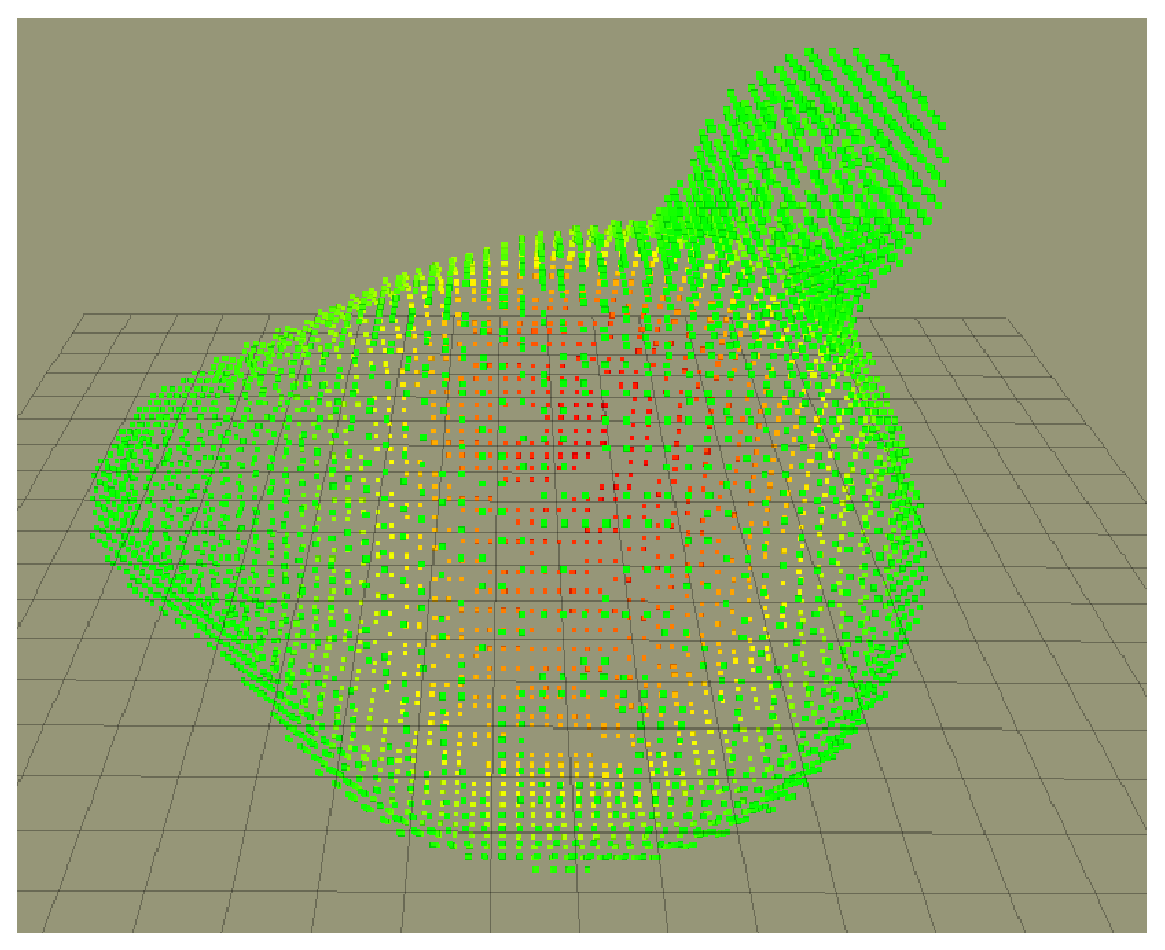
\includegraphics[width=0.45\linewidth]{example.eps}
  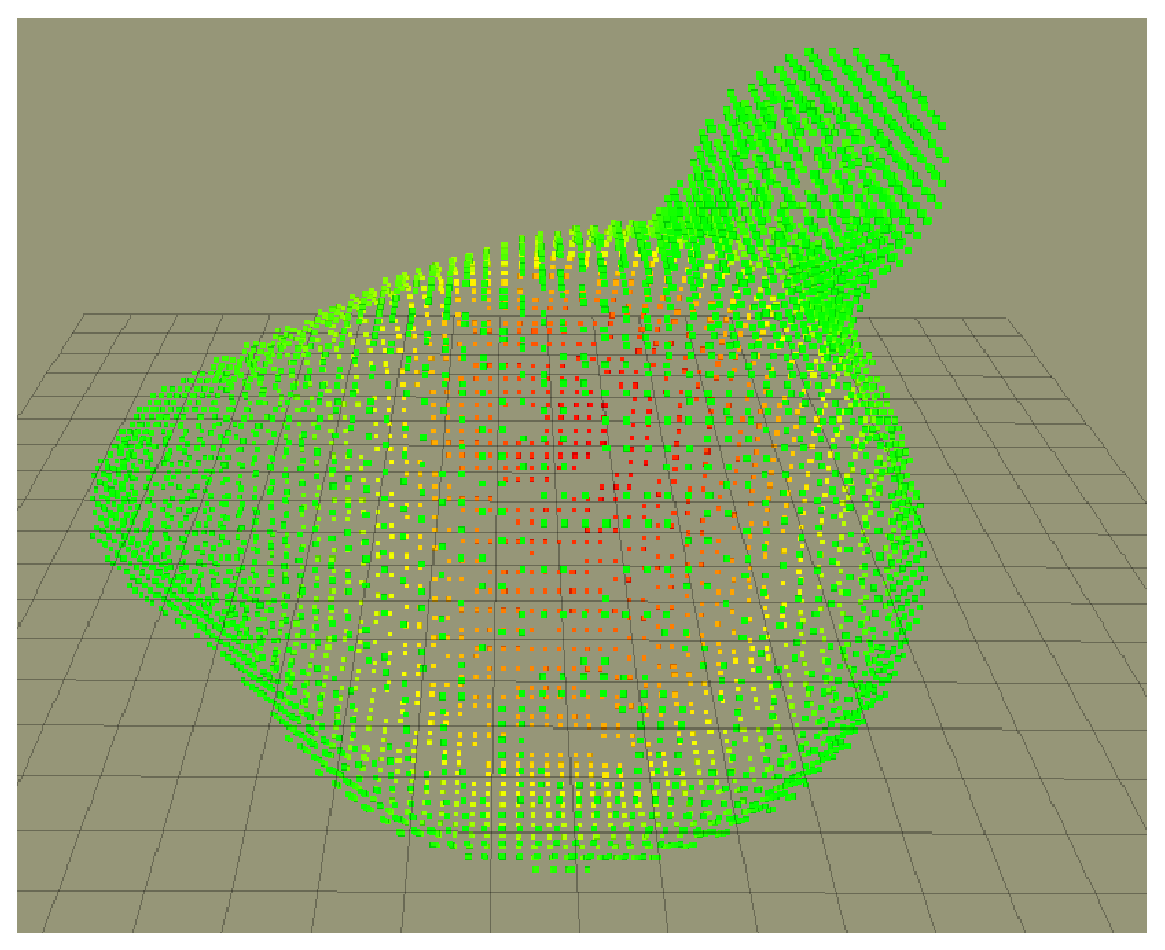
\includegraphics[width=0.45\linewidth]{example.eps}
  }
  \caption{A picture of the in-hand object segmentation using a soft-adaptive hand on a 7-dof arm in the real scene (left) and the resulting point cloud (right).}
  \label{fig:in-hand-segmentation}
\end{figure}

We repeat the exploratory probe given in~\citet{Rosales2014Active}. The probe is composed of a semispherical tip (radius $2$cm) on top of an ATI Nano 17 and an in-parallel passive compliant coupler to safely attach it as the end-effector of a 7 degrees of freedom KUKA LWR 4+ robot arm.

The object is grasped by a the Pisa/IIT SoftHand~\citet{Catalano2014Adaptive}. The assumption that the object is unknown holds to the adaptability of the hand.
There is no need to have a precise model of the object, but a rough approximation of the shape. The hand softness will do the rest. This setup complies with the specifications given in Sect.~\ref{sec:equipment}.



\subsection{Results}
\todo[inline]{To write}

%% This depends on what we use to validate our approach. The easy way is to randomly select a point in space, and go there to touch?


\label{sec:results}
